\chapter{\IfLanguageName{dutch}{Stand van zaken}{State of the art}}
\label{ch:stand-van-zaken}

% Tip: Begin elk hoofdstuk met een paragraaf inleiding die beschrijft hoe
% dit hoofdstuk past binnen het geheel van de bachelorproef. Geef in het
% bijzonder aan wat de link is met het vorige en volgende hoofdstuk.

% Pas na deze inleidende paragraaf komt de eerste sectiehoofding.

Vooraleer we van start kunnen gaan met de diepgaande bespreking van hoe drones een hulpmiddel zijn geweest tijdens de bosbranden in Australië is het niet onbelangrijk om wat onderbouwende informatie te geven over de basiswerking en begrippen van een drone. Er worden voorbeelden van publieke sectoren gegeven waarin drones vaak gebruikt worden alsook in private sectoren. De historiek van drones samen met verschillende types en soorten worden ook als onderbouwende informatie meegegeven. Tot slot wordt er gekeken naar de struikelblokken waarover een drone bezit.

In het tweede luik van dit onderdeel wordt er een algemeen beeld geschetst van de bosbranden in Australië. Hierbij wordt het ontstaan hiervan en de vernieling die het met zich mee bracht besproken.

Tot slot wordt er een kleine inleiding gegeven over de data verzameling en verwerking van een drone.

\section{Wat is een drone?}
\label{sec:wat-zijn-drones}

Een drone of onbemand luchtvaartuig is zoals de naam zegt een luchtvaartuig waarbij een piloot niet nodig is. De drone wordt vanop afstand bestuurd door middel van een afstandsbediening maar kan ook zelfstandig vliegen door het gebruik van voorgeprogrammeerde routes. In het verleden werden deze bijna enkel ingezet voor militaire toepassingen maar in de laatste jaren is er een enorm aanbod aan commerciële drones beschikbaar waardoor deze steeds meer in verschillende sectoren worden gebruikt.

Wanneer er een over een drone wordt gesproken is dit een vrij breed begrip, er zijn op dit moment namelijk al talloze verschillende types en soorten drones. Enkele belangrijke begrippen en onderverdelingen voor drones zijn als volgt:

\textbf{Drone}

Dit is de algemene en ingeburgerde term die wordt gebruikt door het Algemeen Nederlands Woordenboek. Het woordenboek\textcite{VanDale2020} beschrijft een drone als \textit{luchtvaartuig zonder piloot aan boord; onbemand vliegtuigje}. Deze term heeft zijn herkomst van de Engelstalige benaming voor een mannelijke bij n.l. drone (dar in het Nederlands). Deze verwijzing is ontstaan omdat een mannelijke bij in vlucht nagenoeg hetzelfde geluid maakt als een drone. Het is ook deze term die doorheen deze scriptie het meest zal gebruikt worden.

\textbf{UAV en UAS}

Dit zijn twee Engelstalige termen die naast drone wat meer in detail treden over het geheel. De afkorting UAV staat voor \textit{Unmanned Aerial Vehicle} waarbij het eigenlijke vliegend toestel wordt bedoeld dat rond vliegt en data en afbeeldingen verzamelt. Met de term UAS, wat staat voor 'Unmanned Aerial System' bedoeld men het volledige pakket dat nodig is voor gebruik. Hieronder valt de UAV, maar ook het beheersysteem op grondniveau, de camera, GPS, systeemsoftware en de nodige apparatuur om onderhoud uit te voeren. \autocite{Jurovich2017}

\textbf{RPAS}

Een andere term die wordt gebruikt om over een drone te spreken is RPAS, wat staat voor \textit{Remotely Piloted Aircraft Systems}. Het verschil dat hierin wordt gemaakt in vergelijking met een gewone drone, is dat dit enkel gaat over drones die niet-autonoom vliegen. Als er wordt gesproken over een drone kan dit ook inhouden dat deze autonoom bestuurd wordt, wat inhoudt zonder tussenkomst van een piloot.

\textbf{Andere terminologie}

Uiteraard zijn er nog veel andere termen om drones te benoemen, dit gaat vaak enkel om kleine verschillen. Enkele voorbeelden van deze andere termen zijn onder andere 'Small Unmanned Aircraft System' (sUAS) en 'Microcopter'.

Mits drones sedert enkele jaren op veel andere vlakken als enkel militair hun plaats hebben gevonden, worden hier voor enkele publieke sectoren voorbeelden gegeven waarop de drone hierin specifiek een verschil maakt.

\textbf{Militaire doeleinden}

Drones worden voor militaire toepassingen al een hele tijd gebruikt. Hier worden ze op grote schaal ingezet als een extra verdediging door vijandelijke gebieden op een veiligere manier te verkennen. Offensieve drones worden ook ingezet waarbij deze over een raket of dergelijke beschikken om vijandelijke doelwitten op een gecontroleerde en veilige manier uit te schakelen.\autocite{Brown2016}


\textbf{Dierenbescherming}

In Afrika is er sinds lange tijd een probleem met stropers die op zoek zijn naar ivoor bij olifanten en neushoorns. Deze dieren worden op jaarbasis massaal geslacht voor deze reden. Een groep genaamd Air Shepherd gebruikt drones om deze stropers te bestrijden. 

Ze laten hun drones over gebieden vliegen en door middel van infrarood camera 's kunnen stropers gemakkelijk opgemerkt worden. Hierna sturen ze boswachters die dichtbij zijn hierop af om ze te arresteren vooraleer ze de dieren kunnen slachten. \autocite{Fieldstadt2015}

\textbf{Agrarische sector}

Ook in de agrarische sector maken drones het leven eenvoudiger, zo introduceerde DJI, een bedrijf dat kwalitatieve drones op de markt brengt, in 2019 de P4 Multispectral. Dit is een drone speciaal gemaakt voor de landbouwsector en kan via 6 ingebouwde camera 's de velden heel nauwkeurig opmeten. Het zorgt ervoor dat er via de drone over de velden kan gevlogen worden en alle gewassen kunnen geïnspecteerd worden. Vervolgens geeft dia via een analyse tool de gezondheid van deze gewassen weer. Het maakt het ook mogelijk om de gezondheid van de bodem op alle plaatsen te meten. Dit maakt het mogelijk om sneller te handelen indien dit nodig is. \autocite{DJI2019}

\textbf{Ziektebestrijding}

Op het moment van het schrijven van deze scriptie heerst er in de wereld een uitbraak van het COVID-19 virus. In China worden drones die origineel waren gebouwd om pesticiden te sprayen in de agrarische sector, omgebouwd zodat deze op openbare plekken oppervlaktes kunnen desinfecteren. Dit maakt het schoonmaken van deze oppervlakten veel sneller en veiliger dan als een persoon dit zou moeten doen.\autocite{Yuang2020}

Door het gevaar van het verspreiden van het COVID-19 virus via menselijk contact worden drones ook ingezet voor het transporten van medische stalen en test benodigdheden. Dit versnelt het proces van transport ook van 20 minuten op conventionele wijze naar 6 minuten via transport met een drone.\autocite{Yuang2020}

Op vlak van de private sector en voor particulieren worden drones onder andere gebruikt in:

\subsection{Historiek}
\label{sec:Historiek}

Als men de letterlijke vertaling van het woord onbemand luchtvaartuig neemt dan dateert de allereerste drone reeds uit het jaar 1849. Het Oostenrijkse leger zat in conflict met Venetië en gebruikte ballonnen waaraan bommen waren vast gemaakt. Aan deze ballonnen hingen eveneens een lont waarmee ze op het juiste moment zouden losgelaten worden. Ze stuurden deze de lucht in met als doel om deze over Venetië te vliegen en het zo te bombarderen. Echter werd er niet genoeg rekening gehouden met de richting van de wind, waardoor deze ballonnen hun doelwit niet bereikten. Ze vlogen door de windrichting in een andere richting, net over andere Oostenrijkse kampen. \autocite{Pumphrey}

We spoelen even door naar 1935, het jaar waarin Reginald Denny, die tevens in die tijd een zeer bekende acteur was, het eerste op afstand bestuurde luchtvaartuig heeft ontwikkeld. Reginald kreeg na de eerste wereldoorlog een enorme interesse in modelvliegtuigen en begon in 1934 een hobby shop hieromtrent. Deze shop groeide al snel uit tot het bedrijf Reginald Denny Industries. Hij had sinds het begin al een visie om op afstand bestuurbare vliegtuigen te maken die dienst konden doen voor het leger en bouwde even later het eerste in zijn soort hiervan. Dit was het RP-1 (Radio-Plane 1), een op afstand bestuurbaar luchtvaartuig van 19kg met een spanwijdte van 3,6m. Dit werd voorgesteld aan het leger, die hiervan erg onder de indruk waren en hij zijn ontwikkelingen kon voortzetten. Hij kwam doorheen de jaren met steeds nieuwe iteraties die voor militaire missies werden gebruikt. \autocite{Guttman2016}

Zie figuur \ref{fig:GeschiedenisDrone}

\begin{figure}[htp]
    \centering
    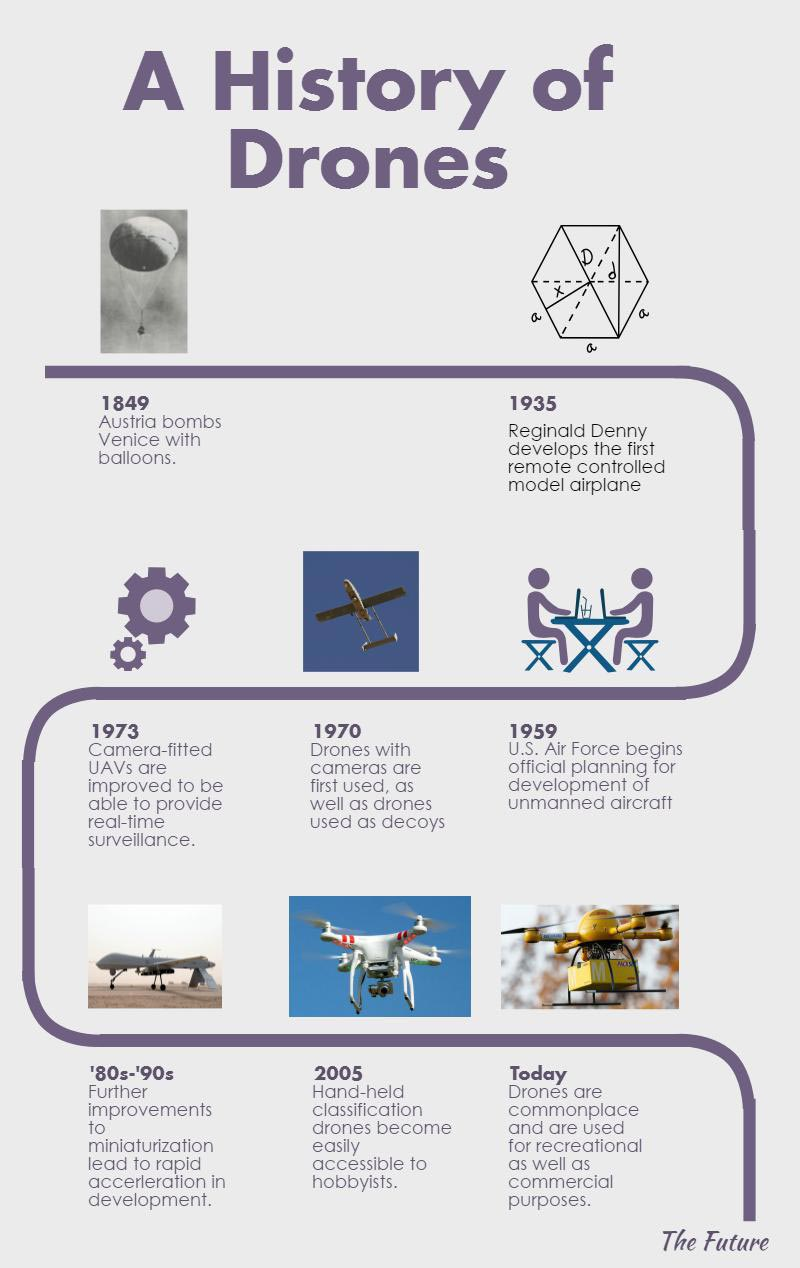
\includegraphics[width=10cm]{bachproef/img/GeschiedenisDrone.jpg}
    \caption{Geschiedenis van drones \autocite{BestRCcopters}}
    \label{fig:GeschiedenisDrone}
\end{figure}

\subsection{Types}
\label{sec:types}

Door de grote opmars die drones in de commerciële sector hebben ondergaan is er op dit moment een breed scala aan beschikbare drones.  

\subsection{Problemen}
\label{sec:problemen}

Natuurlijk zijn er niet enkele positieve aspecten aan het verhaal van de drones, dit brengt ook enkele negatieve zaken met zich mee. Er is het grote debat omtrent privacy bij het gebruik van een drone en hierdoor worden deze aan strikte regels onderworpen. Aangezien een drone een technologisch iets is, is deze ook vatbaar voor mogelijke hacking of het gebruik ervan voor malafide praktijken.

\section{Bosbranden}

Het is zonder twijfel dat iedereen hier reeds op de ene of andere manier op de hoogte van is gebracht. Het was de afgelopen maanden dagelijks in de media en de vernieling die deze branden met zich bracht was op globale schaal ongezien.



